\chapter{Potřebné znalosti sítových protokolů}
\label{chp: network}
Tato kapitola se zaměřuje na~nezbytné znalosti potřebné k~pochopení síťové problematiky. Představuje základní protokoly, jako je \textit{Transmission Control Protocol} (dále označovaný jako \textit{TCP}), jehož role je klíčová při~navazování spojení a~komunikaci. Podrobně vysvětluje \textit{Transport Layer Security} (dále označovaný jako \textit{TLS}), což je protokol pro~standardní zajištění bezpečné komunikace, zejména fázi navázání spojení, poskytující bezpečnostní vlastnosti, strukturu zpráv a~rozdíly verzí \textit{v1.2} a~\textit{v1.3}.

\section{Transmission Control Protocol – TCP}
\label{sec:tcp}
\begin{wrapfigure}{R}{0.33\textwidth}
	\centering
	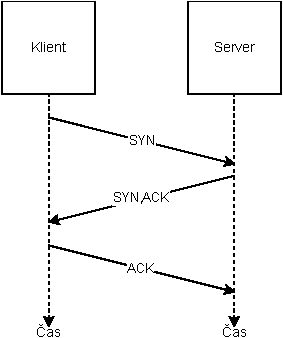
\includegraphics[width=0.33\textwidth]{obrazky-figures/3way-handshake-tcp.pdf}
	\caption{Handshake TCP}
	\label{fig:tcp-handshake}
\end{wrapfigure}
\FloatBarrier

TCP je nejpoužívanějším protokolem \textit{transportní vrstvy} v~sadě protokolů \textit{TCP/IP}, poskytuje spolehlivou službu přenosu dat po~bytech pro~aplikace. Aplikační přenos dat po~bytech je přenášen přes síť prostřednictvím TCP segmentů, přičemž každý TCP segment je odeslán jako datagram protokolu IP (Internet Protocol). Spolehlivost TCP spočívá v~detekci ztráty segmentů (pomocí pořadových čísel) a~chyb (pomocí kontrolních součtů pro~každý segment) a~také v~jejich opravě prostřednictvím opětovného přenosu~\cite{rfc-tcp}. Předtím, než jeden proces může začít posílat data druhému, musí se nejdříve oba vzájemně \uv{domluvit}, tedy provedou takzvaný \textit{handshake}~\cite{kurose2021}. To znamená, že si musí vyměnit několik úvodních segmentů, aby stanovily parametry následného přenosu dat. Handshake obsahuje přesně 3 segmenty. První dva nenesou žádnou zátěž, tedy žádná data aplikační vrstvy, třetí segment ji nést může. Z~počtu segmentů při~ustanovení spojení také vyplývá název \uv{three-way handshake} (\uv{třífázové navázáni spojení} – nadále bude využívána anglická forma, jelikož je to běžné i~mezi~odborníky v~oboru), jak je znázorněno v~diagramu~\ref{fig:tcp-handshake}. Při~komunikaci se pro~ověření správného pořadí segmentů a~případné vyžádání opětovného zaslání ztraceného segmentu používají \textit{sekvenční} (sequence) a~\textit{potvrzovací} (acknowledgment) čísla. Tyto čísla se rovněž používají ve~fázi \textit{three-way handshake}.
\newpage
Navázání spojení probíhá následovně:
\begin{enumerate}
	\item Klient odešle na~server datagram s~příznakem \textit{SYN}\footnote{Synchronize sequence number (česky synchronizace pořadového čísla)}, náhodně vygenerovaným pořadovým číslem $X$ a~potvrzovacím číslem 0.
	\item Server odešle klientovi datagram s~příznaky \textit{SYN} a~\textit{ACK}\footnote{Acknowledgment (česky potvrzení)}, potvrzovacím číslem $X+1$ a~náhodně vygenerovaným pořadovým číslem $Y$. 
	\item Klient dokončuje navázání datagramem s~příznakem \textit{ACK}, pořadovým číslem $X+1$ a~potvrzovacím číslem odpovědi $Y+1$.
\end{enumerate}
Jak již bylo zmíněno, TCP je jedním z~nejpoužívanějších spolehlivých protokolů v~dnešní době. Zajišťuje spolehlivé doručování dat mezi~dvěma koncovými body, avšak má také své neduhy. Jedním z~nejvýraznějších je absence jakéhokoli šifrování, což znamená, že veškerá data přenášená pomocí TCP jsou odesílána v~otevřené, nešifrované podobě. Tato slabina může být využita k~odposlechu nebo manipulaci s~daty, což představuje bezpečnostní riziko. 

Na řadu tedy přichází \textit{TLS} protokol, který poskytuje \textit{šifrování} a~\textit{autenticitu} na~transportní vrstvě\footnote{TLS nelze přesně zařadit k~jedné vrstvě ISO/OSI modelu}, a~tím umožňuje bezpečný přenos aplikačních dat. V~následující podkapitole~\ref{sec:tls} jsou blíže popsány principy fungování a~využití \textit{TLS} v~kombinaci s~\textit{TCP}.

\section{Transport Layer Security – TLS}
\label{sec:tls}
Šifrování, autentizace a~integrita jsou tři zásadní bezpečnostní funkce, které \textit{TCP} postrádá a~\textit{TLS} naopak poskytuje. Tento protokol je nástupcem \textit{SSL}\footnote{Secure Sockets Layer (vrstva bezpečných schránek)}, který byl nahrazen kvůli závažným bezpečnostním chybám a~nedostatečné odolnosti vůči útokům. \textit{TLS} nabízí modernější šifrovací algoritmy a~lepší zabezpečení, čímž překonává nedostatky \textit{SSL}. V~dnešní době je \textit{SSL} prakticky historií, a~proto se tato práce zaměřuje výhradně na~komunikaci pomocí \textit{TLS}. Vzhledem k~tomu, že v~poskytnutých datových sadách, jak je zmíněno v~sekci~\ref{sec:dataset}, se převážně objevuje \textit{TLS} \textbf{verze 1.2}, bude pozornost této sekce věnována právě této verzi.

Protokol se skládá ze dvou vrstev: \textit{TLS Record Protocol} a~\textit{TLS Handshake Protocol}. \textit{Record Protokol} zapouzdřuje různé protokoly vyšších vrstev. Jeden z~těchto zapouzdřených protokolů je \textit{TLS Handshake}, který umožňuje serveru a~klientovi vzájemnou autentizaci a~vyjednání šifrovacích algoritmů a~kryptografických klíčů před~zahájením komunikace aplikačních protokolů.

\textit{TLS Record Protocol} následně přebírá data aplikační vrstvy, která mají být přenesena. Operuje nad~těmito daty, která jsou nejprve fragmentována, případně komprimována, je k~nim přidán kód MAC (Message Authentication Code\,--\,kód autentizace zprávy), poté jsou zašifrována a~přidána hlavička protokolu. Takto vytvořená datová jednotka je poté předána do~TCP segmentu pro~přenos~\cite{Stallings2017}.


Jednou z~výhod je skutečnost, že \textit{TLS} je nezávislý na~aplikačním protokolu a~datech aplikační úrovně, které šifruje. Protokoly vyšší úrovně mohou na~něj navazovat \textbf{transparentně}. Kromě snad nejpoužívanějšího aplikačního protokolu HTTP se TLS využívá také pro~protokoly jako například \textit{FTP}, \textit{SMTP}, \textit{NNTP} a~další. TLS není omezeno pouze na~funkčnost nad~TCP, ale dokáže zabezpečit komunikaci stejně přes \textit{UDP} či \textit{DCCP}. Díky již zmíněné transparentnosti vůči přenášenému aplikačnímu protokolu může také poskytovat zabezpečení při~VPN spojení, typicky v~případě použití \textit{OpenConnect} nebo \textit{OpenVPN}~\cite{rfc-sec_proto}. Další možností využití je při~e-mailové komunikaci pomocí příkazu \textit{STARTTLS}~\cite{matousek2014}.

Standard však nespecifikuje, jak protokoly implementují zabezpečení pomocí \textit{TLS}. Rozhodnutí o~tom, jak zahájit \textit{handshake} a~jak interpretovat autentizační certifikáty, které jsou vyměněny, jsou ponechána na~uvážení návrhářů a~vývojářů protokolů operujících nad~\textit{TLS}~\cite{rfc-tls12}. 

Dle \textit{ISO/OSI} modelu nelze protokol \textit{TLS} správně klasifikovat, jelikož operuje především nad~\textit{TCP}, které se nachází ve~4. vrstvě, a~samotné \textit{TLS} poskytuje bezpečné navázání a~udržení relace, při~fázi \textit{handshake}, což je funkce 5. vrstvy (\textit{relační}). Zároveň šifruje aplikační data, což je funkcí prezentační vrstvy. Z~pohledu šifrování, které je hlavní funkcí, lze \textit{TLS} nejlépe zařadit do~6. vrstvy (\textit{prezentační}). Nicméně klasifikace \textit{TLS} pouze do~jedné vrstvy není přesná, protože plní funkce napříč několika vrstvami modelu \textit{ISO/OSI}.

\subsection{Základní bezpečnostní funkce}

Tato podkapitola, převzata a~upravena z~\cite{rfc-tls12}, se zaměřuje na~základní bezpečnostní funkce protokolu TLS, konkrétně na~symetrickou kryptografii, integritu dat a~autentizaci, které společně zajišťují bezpečnost komunikace.

\subsubsection{Důvěrnost}
Symetrická kryptografie je základní metodou pro~šifrování přenášených dat. Pro~šifrování se používají různé algoritmy, jako je \textit{AES} (Advanced Encryption Standard), který je v~dnešní době považován za~velmi bezpečný a~široce používaný. Starší algoritmy, jako \textit{RC4}, byly dříve běžně nasazovány, ale kvůli nalezeným zranitelnostem a~slabinám jsou již považovány za~zastaralé a~jejich použití se nedoporučuje~\cite{rfc-rc4}.

Důvěrnost je zajištěna tím, že klíče používané pro~šifrování jsou unikátně generovány pro~každou relaci (tzv.~\uv{session}). Tyto klíče se odvozují z~tajemství, které je bezpečně vyjednáno během \textit{handshake} fáze. Nejběžněji používanými metodami jsou výměny klíčů na~bázi algoritmů \textit{Diffie-Hellman} a~\textit{RSA}, který se používá pro~asymetrické šifrování. Protokol \textit{TLS} rovněž umožňuje komunikaci bez~šifrování, což však odporuje hlavnímu účelu protokolu.

\subsubsection{Integrita dat}
Kontrola integrity je klíčová pro~zajištění, že data nebyla během přenosu pozměněna třetí stranou. Přenos zpráv zahrnuje kontrolu integrity zpráv pomocí hodnoty \textit{MAC}. Pro~výpočet MAC se používají bezpečné hašovací algoritmy, jako je \textit{SHA-256}, který se stal standardem pro~moderní aplikace. Starší algoritmy, jako je \textit{MD5} a~\textit{SHA-1}, byly dříve široce používány, ale kvůli objevení kolizí a~zranitelností se již nedoporučují~\cite{sha-collision}.

\subsubsection{Autentizace}
Autentizace se nejčastěji provádí pomocí asymetrické kryptografie. Servery se autentizují vůči klientům pomocí digitálních certifikátů, které obsahují veřejný klíč serveru a~jsou podepsány důvěryhodnou certifikační autoritou (CA). Autentizace klientů je volitelná, ale v~některých případech, například v~případě přístupu k~citlivým systémům, může být požadována. Nejčastěji se používají algoritmy jako \textit{RSA} nebo \textit{ECDSA}.

Tyto základní bezpečnostní funkce symetrické kryptografie, integrity dat a~autenticity společně zajišťují důvěryhodnost a~bezpečnost moderní internetové komunikace, čímž umožňují uživatelům důvěřovat přenášeným informacím.

\subsection{Navázání spojení}

Počátkem každé komunikace je navázání spojení mezi~účastníky. U~TLS tomu není jinak a, jak již bylo zmíněno, tato fáze se nazývá \uv{TLS handshake}. Po~navázání a~ustanovení spojení protokolem \textit{TCP}, k~čemuž slouží \textit{three-way handshake}, jenž je podrobně rozepsán v~\ref{sec:tcp}, se \textit{TLS} pokusí navázat bezpečné spojení a~vyjednat detaily budoucí komunikace. Pro~lepší představu je znázorněno diagramem~\ref{fig:tls-handshake}.

\begin{wrapfigure}{R}{0.33\textwidth}
	\centering
	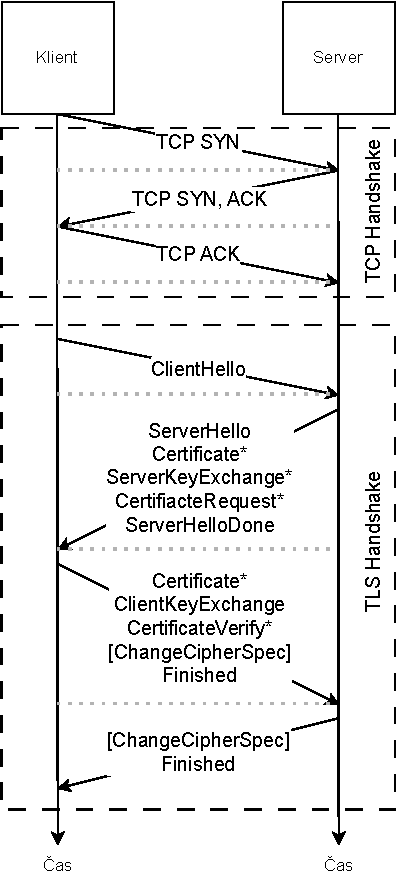
\includegraphics[width=0.33\textwidth]{obrazky-figures/tls-handshake.pdf}
	\caption{Handshake TLS}
	\label{fig:tls-handshake}
\end{wrapfigure}
\FloatBarrier

Postup ustanovení spojení mezi~klientem a~serverem probíhá následovně:
\begin{enumerate}
	\item Klient zašle zprávu \textit{ClientHello}, obsahující seznam kryptografických algoritmů, které podporuje, spolu s~náhodně vygenerovaným číslem (označovaným jako \uv{nonce}\footnote{Kryptografická nonce je označení pro~náhodné číslo, které lze použít pouze jednou. Jeho přítomnost zvyšuje obtížnost podvržení zprávy.}).
	\item Ze seznamu je serverem vybrán algoritmus pro~\textbf{symetrickou} kryptografii, algoritmus pro~\textbf{asymetrickou} kryptografii a~typ \textbf{\textit{HMAC}} (Hash-based Message Authentication Code, česky autentizační kód zprávy). Dále je zvolena \textbf{hašovací funkce}, např. \textit{MD5}, \textit{SHA-2},\dots Vybrané algoritmy jsou zaslány zpět klientovi spolu s~certifikátem serveru a~náhodně vygenerovaným číslem (nonce), jako součást zprávy \textit{Server Hello}.
	\item Klient ověří certifikát, získá veřejný klíč serveru, vygeneruje \textit{Pre-Master Secret} (dále označovaný jako \uv{PMS}), zašifruje \textit{PMS} veřejným klíčem serveru a~odešle šifrovaný \textit{PMS} serveru.
	\item Pomocí stejné funkce pro~odvození klíče, jak je stanoveno standardem \textit{TLS}~\cite{rfc-tls12}, klient a~server nezávisle vypočítají \textit{Master Secret} (dále označovaný jako \uv{MS}) z~\textit{PMS} a~nonce. \textit{MS} se poté rozdělí na~dva šifrovací klíče a~dva \textit{HMAC} klíče. Dále, pokud vybraný symetrický šifrovací algoritmus používá režim \textit{CBC} (Cipher Block Chaining, česky \uv{Řetězení šifrovacích bloků}, a~dále označován zkratkou \textit{CBC}), například \textit{3DES} nebo \textit{AES}, jsou z~\textit{MS} získány také dva inicializační vektory (\textit{IV}) --jeden pro~každou stranu spojení. Následně jsou všechny zprávy mezi~klientem a~serverem šifrovány a~autentizovány (pomocí \textit{HMAC}). Obě strany si vzájemně zašlou \textit{HMAC} vypočítaný na~základě všech předchozích zpráv, aby ověřily integritu celé fáze navazování a~vyjednávání spojení.
\end{enumerate}

Proces navazování spojení, odehrávající se v~5.vrstvě (\textit{relační}) \textit{ISO/OSI} modelu, pomocí protokolu \textit{TLS Handshake} je klíčovým prvkem k~zajištění bezpečné komunikace mezi~dvěma stranami. Správný výběr algoritmů a~hašovacích funkcí, ověřování HMAC a~použití nonce jsou zásadní pro~ochranu dat a~zajištění důvěrnosti. V~další podsekci~\ref{sec:clienthello} je podrobně popsán obsah těchto zpráv, které nejsou šifrovány a~využívají se k~tvorbě TLS otisku. Bližší popis TLS otisku je v~kapitole~\ref{chp:JA34}.

\subsection{Obsah zprávy Client Hello}
\label{sec:clienthello}
V této podsekci je popsán obsah zpráv \textit{Client Hello}. Následující struktura\textit{Client Hello} zpráv je převzata z~\textbf{RFC 5246}~\cite{rfc-tls12}. 

Struktura \textit{Client Hello} je definována následovně:
\begin{verbatim}
struct 
{
    ProtocolVersion client_version;
    Random random;
    SessionID session_id;
    CipherSuite cipher_suites<2..2^16-2>;
    CompressionMethod compression_methods<1..2^8-1>;
    select (extensions_present) 
    {
        case false:
          struct {};
        case true:
          Extension extensions<0..2^16-1>;
    };
} ClientHello;
\end{verbatim}
Kde:
\begin{itemize}
	\item \textbf{client\_version} značí verzi \textit{TLS} protokolu, kterou klient podporuje (např. 771\,--\,pro \textit{TLS v1.2}),
	\item \textbf{random} je klientská nonce,
	\item \textbf{session\_id} označuje identifikátor relace,
	\item \textbf{cipher\_suites} reprezentuje seznam šifrovacích sad podporovaných klientem,
	\item \textbf{compression\_methods} značí seznam metod komprese podporovaných klientem,
	\item \textbf{extensions\_present} indikuje přítomnost rozšíření,
	\item \textbf{extensions}, je kolekce rozšíření poskytujících dodatečné zabezpečení spojení. Běžná rozšíření jsou například \textit{supported\_groups}, které identifikuje eliptické křivky podporované klientem, a~\textit{ec\_point\_formats}, které specifikuje množinu bodů používaných pro~reprezentaci eliptických křivek~\cite{rfc-tls-ext}. Více v~\ref{subsec:ext}.
\end{itemize} 

Zpráva \textit{Client Hello} je zásadním \uv{stavebním kamenem} \textit{TLS} komunikace, protože propaguje možnosti a~vlastnosti klienta, jako jsou podporované verze protokolu, šifrovací sady a~rozšíření. Hodnoty vybraných atributů zprávy  mohou být použity pro~identifikaci pomocí \textit{JA3/JA4} otisků, více viz~\ref{chp:JA34}.


\subsection{Obsah zprávy Server Hello}
\label{sec:serverhello}
Následující struktura \textit{Server Hello} zprávy je převzata z~\textbf{RFC 5246}~\cite{rfc-tls12}. Struktura zprávy \textit{Server Hello} je následující:

\begin{verbatim}
struct 
{
    ProtocolVersion server_version;
    Random random;
    SessionID session_id;
    CipherSuite cipher_suite;
    CompressionMethod compression_method;
    select (extensions_present) 
    {
        case false:
          struct {};
        case true:
          Extension extensions<0..2^16-1>;
    };
} ServerHello;
\end{verbatim}
Kde:
\begin{itemize}
	\item \textbf{server\_version} značí verzi \textit{TLS} protokolu, kterou server vybral na~základě \textit{client\_version},
	\item \textbf{random} je nonce serveru,
	\item \textbf{session\_id} označuje identifikátor relace,
	\item \textbf{cipher\_suite} reprezentuje jednu šifrovací sadu vybranou z~\textit{cipher\_suites},
	\item \textbf{compression\_method} značí jednu metodu komprese zvolenou serverem,    
	\item \textbf{extensions\_present} indikuje přítomnost rozšíření,
	\item \textbf{extensions}, stejně jako u~\textit{Client Hello}, určuje jaká rozšíření vybraná serverem jsou podporována. Více v~\ref{subsec:ext}.
\end{itemize}

Výběr z~výše zmíněných elementů zpráv je využit pro~tvorbu a~následnou identifikaci pomocí \textit{JA3/JA4} otisků, jak je detailněji popsáno dále v~kapitole~\ref{chp:JA34}. V~následující podsekci~\ref{sec:tls-13} jsou rozepsány podrobnosti implementace \textit{TLS} verze \textit{1.3} a~také jsou zmíněny změny \textit{Hello} zpráv oproti verzi \textit{1.2}. 

\subsection{Možná rozšíření}
\label{subsec:ext}
Detailní popis všech možných atributů a~funkcí těchto zpráv je nad~rámec této technické zprávy. Proto jsou uvedeny pouze potřebné informace pro~pochopení a~následné vysvětlení v~kontextu s~\textit{JA3} a~\textit{JA4} otisky. Z~tohoto důvodu jsou zde uvedena pouze nejčastější a~informačně nejvýznamnější rozšíření, která jsou používána k~tvorbě otisků nebo ke~zlepšení přesnosti identifikace.

\begin{itemize}
	\item \textbf{Server Name Indicator} (\textit{Indikátor jména serveru}, dále jen \uv{SNI}) umožňuje klientům poskytnout název serveru, se kterým se spojují. Tato funkce je žádoucí pro~usnadnění zabezpečených připojení k~serverům, které provozují více \uv{virtuálních} serverů na~jedné adrese~\cite{rfc-sni}.
	      	          
	\item \textbf{Application-Layer Protocol Negotiation} (\textit{Vyjednání aplikačního protokolu}, dále jen \uv{ALPN}) V~situaci, kdy je na~jednom portu serveru, například portu 443, podporováno více aplikačních protokolů, klient a~server musí vyjednat aplikační protokol, který bude použit pro~každé připojení. S~\textit{ALPN} klient odesílá seznam podporovaných aplikačních protokolů jako součást zprávy \textit{TLS Client Hello}. Server si vybere protokol a~odešle vybraný protokol jako součást zprávy \textit{TLS Server Hello}~\cite{rfc-alpn}. Vyjednávání aplikačního protokolu tak může být provedeno v~rámci protokolu \textit{handshake}, aniž by se přidávaly další síťové výměny, a~umožňuje serveru přiřadit k~jednotlivým aplikačním protokolům různé certifikáty.
	      	      
\end{itemize}

\subsection{TLS verze 1.3}
\label{sec:tls-13}
\textit{TLS verze 1.3} je \textbf{nejnovější} verzí protokolu \textit{TLS}. Mezi~nejvýznamnější rozdíly posledních dvou verzí patří především změny v~seznamu povolených šifer u~symetrické kryptografie, kde v~novější verzi zůstávají pouze \textbf{AEAD} (\textit{Authenticated Encryption with Associated Data} -- česky autentizované šifrování s~připojenými daty) algoritmy. \textit{Handshake} protokol je zrychlen pomocí techniky \textbf{0-RTT} (\textit{Zero Round-Trip Time} -- česky nulová doba navázání spojení), která šetří jednu cestu tam a~zpátky na~úkor některých bezpečnostních vlastností. Nová verze také \textbf{šifruje} všechny zprávy protokolu \textit{Handshake} po~zprávě \textit{Server Hello}~\cite{rfc-tls13}. Plánuje se také začít šifrovat \textit{Hello} zprávy, čímž se znemožní identifikaci pomocí pouhých \textit{JA3}/\textit{JA4} otisků~\cite{encrypted-hello}.

Také byly představeny takzvané \textbf{GREASE} (\textit{Generate Random Extensions And Sustain Extensibility}) hodnoty, které jsou přidávány do~atributů zpráv handshake protokolu, k~ověření správné implementace protější strany. Při~správném zpracování musí být tyto hodnoty ignorovány druhou stranou. V~případě, že \textit{GREASE} hodnoty nejsou tolerovány, je vyhlášena chyba, která značí nevalidní implementaci~\cite{rfc-grease}.

\textit{TLS} je typicky implementován nad~\textit{TCP} protokolem, ovšem verze 1.3 dokáže komunikovat také přes \textit{UDP} (\textit{User Datagram Protocol}) v~případě, že je použit protokolem \textbf{QUIC} (\textit{Quick UDP Internet Connections}). \textit{QUIC} využívá \textit{UDP} jako transportní protokol a~zároveň na~něm staví pokročilé funkce, jako je správa spojení a~zajištění spolehlivosti~\cite{rfc-quic}. Má zabudované zabezpečení pomocí \textit{TLS v1.3}, díky čemuž poskytuje všechny bezpečnostní výhody \textit{TLS}~\cite{rfc-quic-tls}.
